\subsection{Know about}

El usuario necesitara saber que tiene este recurso y puede utilizarlo ya que aunque optimicemos la represantacion del 
conjunto de datos y lo ofrezcamos a los usuarios, este no sera util si los usuarios no son conscientes de que existe.
\subsubsection{How to solve it} 
La mejor manera es publicitando el producto en los medios y entorno adecuado.
\subsubsection{How we solve it. Aire Guru} 
Nuestra herramienta esta implementada para la ciudad de Malaga, por lo que actualmente se esta trabajando para darla a 
conocer en esta ciudad.
De momento esta disponible en el portal de datos abiertos en la pestana de aplicaciones\footnote{\url{https://datosabiertos.malaga.eu/aplicaciones}}\\
Participo en el primer concurso de reutilizacion datos abiertos organizado por el Ayuntamiento de Malaga \footnote{\url{https://tinyurl.com/yx9wzutj}}
quedando finalista en la categoria de pagina web.

aireGuruFinalist

\begin{figure}[ht]
    \centering
   \subfigure[Publicidad en el portal de datos abiertos de Malaga]{ \centering 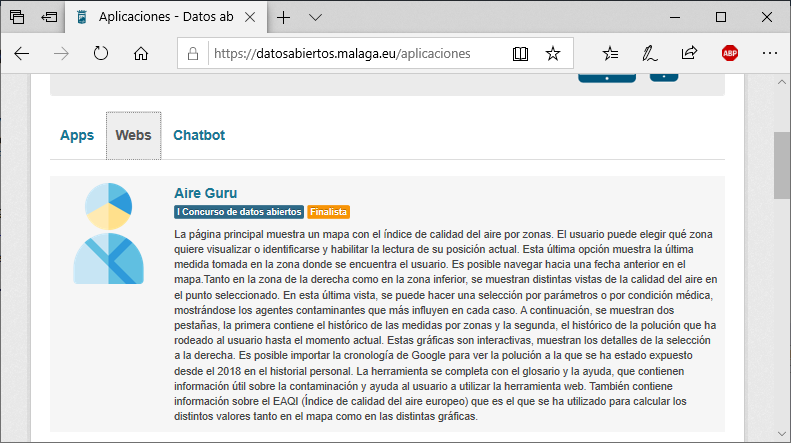
\includegraphics[width=6cm]{aireGuruFinalist}}
   \hfill
   \subfigure[Finalist]{ \centering 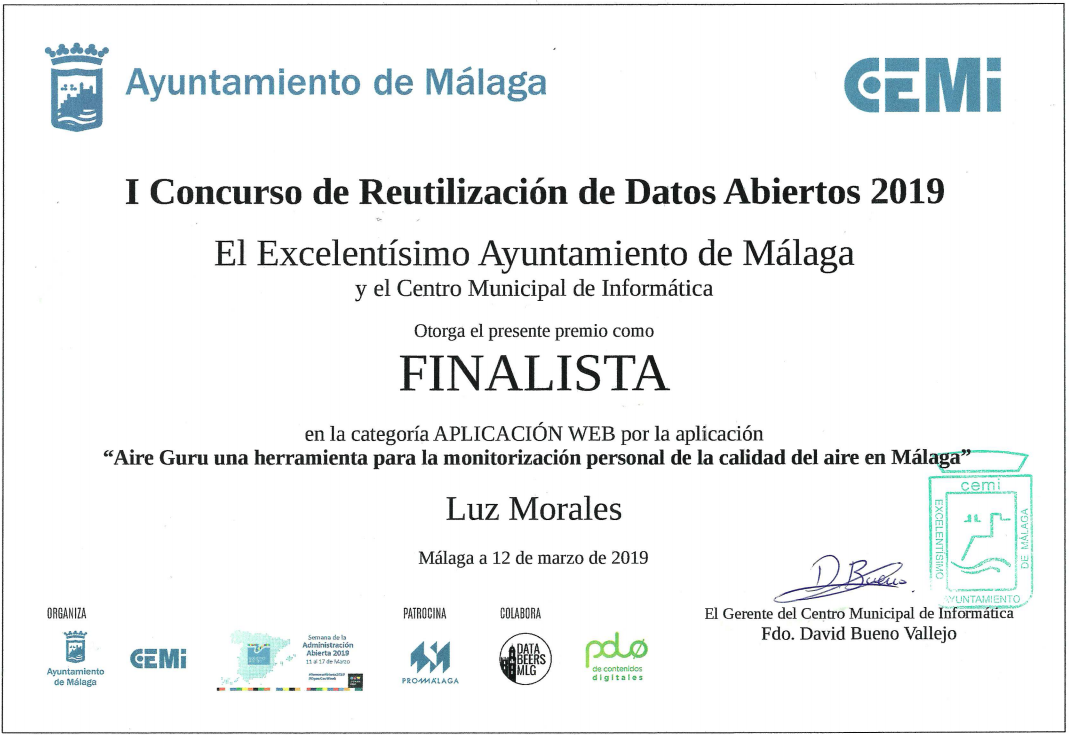
\includegraphics[width=5cm]{aireGuruFinalistCertificate}}
 
    \caption{I Concurso de reutilizacion de datos abiertos. Ayuntamiento de Malaga}
    \end{figure}

\elsparagraph{Evaluation}  
\begin{itemize}
\done Actualmente esta publicado en el portal de datos abiertos del Ayuntamiento de Malaga.
\crossed Deberia trabajarse mas en la publicidad de la plataforma y darla a conocer.  
\end{itemize}
\newpage